%%%%%%%%%%%%%%%%%%%%%%%%%%%%%%%%%%%%%%%%%%%%%%%%%%%%%%%%%%%%%%%%%%%%%%
%%  disstemplate.tex, to be compiled with latex.		     %
%%  08 April 2002	Version 4				     %
%%%%%%%%%%%%%%%%%%%%%%%%%%%%%%%%%%%%%%%%%%%%%%%%%%%%%%%%%%%%%%%%%%%%%%
%%								     %
%%  Writing a Doctoral Dissertation with LaTeX at		     %
%%	the University of Texas at Austin			     %
%%								     %
%%  (Modify this ``template'' for your own dissertation.)	     %
%%								     %
%%%%%%%%%%%%%%%%%%%%%%%%%%%%%%%%%%%%%%%%%%%%%%%%%%%%%%%%%%%%%%%%%%%%%%


\documentclass[12pt]{report}	% The documentclass must be ``report''.

\usepackage{utdiss2}  		% Dissertation package style file.
\usepackage{listings}


%%%%%%%%%%%%%%%%%%%%%%%%%%%%%%%%%%%%%%%%%%%%%%%%%%%%%%%%%%%%%%%%%%%%%%
% Optional packages used for this sample dissertation. If you don't  %
% need a capability in your dissertation, feel free to comment out   %
% the package usage command.					     %
%%%%%%%%%%%%%%%%%%%%%%%%%%%%%%%%%%%%%%%%%%%%%%%%%%%%%%%%%%%%%%%%%%%%%%

\usepackage{amsmath,amsthm,amsfonts,amscd} 
				% Some packages to write mathematics.
\usepackage{eucal} 	 	% Euler fonts
\usepackage{verbatim}      	% Allows quoting source with commands.
\usepackage{makeidx}       	% Package to make an index.
\usepackage{psfig}         	% Allows inclusion of eps files.
\usepackage{epsfig}         	% Allows inclusion of eps files.
\usepackage{citesort}         	% 
\usepackage{url}		% Allows good typesetting of web URLs.
%\usepackage{draftcopy}		% Uncomment this line to have the
				% word, "DRAFT," as a background
				% "watermark" on all of the pages of
				% of your draft versions. When ready
				% to generate your final copy, re-comment
				% it out with a percent sign to remove
				% the word draft before you re-run
				% Makediss for the last time.

\author{Cassidy Aaron Burden}  	% Required

\address{1015 Strickland Dr.\\ Austin, Texas 78748}  % Required

\title{Evaluating Headroom for Hawkeye and Precleaning on GPUs}
                                                    % Required

%%%%%%%%%%%%%%%%%%%%%%%%%%%%%%%%%%%%%%%%%%%%%%%%%%%%%%%%%%%%%%%%%%%%%%
% NOTICE: The total number of supervisors and other members %%%%%%%%%%
%%%%%%%%%%%%%%% MUST be seven (7) or less! If you put in more, %%%%%%%
%%%%%%%%%%%%%%% they are put on the page after the Committee %%%%%%%%%
%%%%%%%%%%%%%%% Certification of Approved Version page. %%%%%%%%%%%%%%
%%%%%%%%%%%%%%%%%%%%%%%%%%%%%%%%%%%%%%%%%%%%%%%%%%%%%%%%%%%%%%%%%%%%%%

%%%%%%%%%%%%%%%%%%%%%%%%%%%%%%%%%%%%%%%%%%%%%%%%%%%%%%%%%%%%%%%%%%%%%%
%
% Enter names of the supervisor and co-supervisor(s), if any,
% of your dissertation committee. Put one name per line with
% the name in square brackets. The name on the last line, however,
% must be in curly braces.
%
% If you have only one supervisor, the entry below will read:
%
%	\supervisor
%		{Supervisor's Name}
%
% NOTE: Maximum three supervisors. Minimum one supervisor.
% NOTE: The Office of Graduate Studies will accept only two supervisors!
% 
%
\supervisor
	{Calvin Lin}

%%%%%%%%%%%%%%%%%%%%%%%%%%%%%%%%%%%%%%%%%%%%%%%%%%%%%%%%%%%%%%%%%%%%%%
%
% Enter names of the other (non-supervisor) members(s) of your
% dissertation committee. Put one name per line with the name
% in square brackets. The name on the last line, however, must
% be in curly braces.
%
% NOTE: Maximum six other members. Minimum zero other members.
% NOTE: The Office of Graduate Studies may restrict you to a total
%	of six committee members.
%
%
\committeemembers
	{Akanksha Jain}

%%%%%%%%%%%%%%%%%%%%%%%%%%%%%%%%%%%%%%%%%%%%%%%%%%%%%%%%%%%%%%%%%%%%%%

\previousdegrees{B.S.}
     % The abbreviated form of your previous degree(s).
     % E.g., \previousdegrees{B.S., MBA}.
     %
     % The default value is `B.S., M.S.'

\graduationmonth{May}      
     % Graduation month, either May, August, or December, in the form
     % as `\graduationmonth{May}'. Do not abbreviate.
     %
     % The default value (either May, August, or December) is guessed
     % according to the time of running LaTeX.

%\graduationyear{...}   
     % Graduation year, in the form as `\graduationyear{2001}'.
     % Use a 4 digit (not a 2 digit) number.
     %
     % The default value is guessed according to the time of 
     % running LaTeX.

%\typist{...}       
     % The name(s) of typist(s), put `the author' if you do it yourself.
     % E.g., `\typist{Maryann Hersey and the author}'.
     %
     % The default value is `the author'.


%%%%%%%%%%%%%%%%%%%%%%%%%%%%%%%%%%%%%%%%%%%%%%%%%%%%%%%%%%%%%%%%%%%%%%
% Commands for master's theses and reports.			     %
%%%%%%%%%%%%%%%%%%%%%%%%%%%%%%%%%%%%%%%%%%%%%%%%%%%%%%%%%%%%%%%%%%%%%%
%
% If the degree you're seeking is NOT Doctor of Philosophy, uncomment
% (remove the % in front of) the following two command lines (the ones
% that have the \ as their second character).
%
\degree{MASTER OF SCIENCE IN ENGINEERING}
\degreeabbr{M.S.E.}

% Uncomment the line below that corresponds to the type of master's
% document you are writing.
%
\masterreport
%\masterthesis


%%%%%%%%%%%%%%%%%%%%%%%%%%%%%%%%%%%%%%%%%%%%%%%%%%%%%%%%%%%%%%%%%%%%%%
% Some optional commands to change the document's defaults.	     %
%%%%%%%%%%%%%%%%%%%%%%%%%%%%%%%%%%%%%%%%%%%%%%%%%%%%%%%%%%%%%%%%%%%%%%
%
%\singlespacing
%\oneandonehalfspacing

%\singlespacequote
\oneandonehalfspacequote

\topmargin 0.125in	% Adjust this value if the PostScript file output
			% of your dissertation has incorrect top and 
			% bottom margins. Print a copy of at least one
			% full page of your dissertation (not the first
			% page of a chapter) and measure the top and
			% bottom margins with a ruler. You must have
			% a top margin of 1.5" and a bottom margin of
			% at least 1.25". The page numbers must be at
			% least 1.00" from the bottom of the page.
			% If the margins are not correct, adjust this
			% value accordingly and re-compile and print again.
			%
			% The default value is 0.125"

		% If you want to adjust other margins, they are in the
		% utdiss2-nn.sty file near the top. If you are using
		% the shell script Makediss on a Unix/Linux system, make
		% your changes in the utdiss2-nn.sty file instead of
		% utdiss2.sty because Makediss will overwrite any changes
		% made to utdiss2.sty.

%%%%%%%%%%%%%%%%%%%%%%%%%%%%%%%%%%%%%%%%%%%%%%%%%%%%%%%%%%%%%%%%%%%%%%
% Some optional commands to be tested.				     %
%%%%%%%%%%%%%%%%%%%%%%%%%%%%%%%%%%%%%%%%%%%%%%%%%%%%%%%%%%%%%%%%%%%%%%

% If there are 10 or more sections, 10 or more subsections for a section,
% etc., you need to make an adjustment to the Table of Contents with the
% command \longtocentry.
%
%\longtocentry 



%%%%%%%%%%%%%%%%%%%%%%%%%%%%%%%%%%%%%%%%%%%%%%%%%%%%%%%%%%%%%%%%%%%%%%
%	Some math support.					     %
%%%%%%%%%%%%%%%%%%%%%%%%%%%%%%%%%%%%%%%%%%%%%%%%%%%%%%%%%%%%%%%%%%%%%%
%
%	Theorem environments (these need the amsthm package)
%
%% \theoremstyle{plain} %% This is the default

\newtheorem{thm}{Theorem}[section]
\newtheorem{cor}[thm]{Corollary}
\newtheorem{lem}[thm]{Lemma}
\newtheorem{prop}[thm]{Proposition}
\newtheorem{ax}{Axiom}

\theoremstyle{definition}
\newtheorem{defn}{Definition}[section]

\theoremstyle{remark}
\newtheorem{rem}{Remark}[section]
\newtheorem*{notation}{Notation}

%\numberwithin{equation}{section}


%%%%%%%%%%%%%%%%%%%%%%%%%%%%%%%%%%%%%%%%%%%%%%%%%%%%%%%%%%%%%%%%%%%%%%
%	Macros.							     %
%%%%%%%%%%%%%%%%%%%%%%%%%%%%%%%%%%%%%%%%%%%%%%%%%%%%%%%%%%%%%%%%%%%%%%
%
%	Here some macros that are needed in this document:


\newcommand{\latexe}{{\LaTeX\kern.125em2%
                      \lower.5ex\hbox{$\varepsilon$}}}

\newcommand{\amslatex}{\AmS-\LaTeX{}}

\chardef\bslash=`\\	% \bslash makes a backslash (in tt fonts)
			%	p. 424, TeXbook

\newcommand{\cn}[1]{\texttt{\bslash #1}}

\makeatletter		% Starts section where @ is considered a letter
			% and thus may be used in commands.
\def\square{\RIfM@\bgroup\else$\bgroup\aftergroup$\fi
  \vcenter{\hrule\hbox{\vrule\@height.6em\kern.6em\vrule}%
                                              \hrule}\egroup}
\makeatother		% Ends sections where @ is considered a letter.
			% Now @ cannot be used in commands.

\makeindex    % Make the index

%%%%%%%%%%%%%%%%%%%%%%%%%%%%%%%%%%%%%%%%%%%%%%%%%%%%%%%%%%%%%%%%%%%%%%
%		The document starts here.			     %
%%%%%%%%%%%%%%%%%%%%%%%%%%%%%%%%%%%%%%%%%%%%%%%%%%%%%%%%%%%%%%%%%%%%%%

\begin{document}

\copyrightpage          % Produces the copyright page.


%
% NOTE: In a doctoral dissertation, the Committee Certification page
%		(with signatures) is BEFORE the Title page.
%	In a masters thesis or report, the Signature page
%		(with signatures) is AFTER the Title page.
%
%	If you are writing a masters thesis or report, you MUST REVERSE
%	the order of the \commcertpage and \titlepage commands below.
%
			%   of Approved Version page (doctoral)
			%   or Signature page (masters).
			%		20 Mar 2002	cwm

\titlepage              % Produces the title page.
\commcertpage           % Produces the Committee Certification



%%%%%%%%%%%%%%%%%%%%%%%%%%%%%%%%%%%%%%%%%%%%%%%%%%%%%%%%%%%%%%%%%%%%%%
% Dedication and/or epigraph are optional, but must occur here.      %
%%%%%%%%%%%%%%%%%%%%%%%%%%%%%%%%%%%%%%%%%%%%%%%%%%%%%%%%%%%%%%%%%%%%%%
%
%\begin{dedication}
%\index{Dedication@\emph{Dedication}}%
%Dedicated to my wife Shirley.
%\end{dedication}


%\begin{acknowledgments}		% Optional
%\index{Acknowledgments@\emph{Acknowledgments}}%
%I wish to thank the multitudes of people who helped me. Time would
%fail me to tell of \ldots
%\end{acknowledgments}


% The abstract is required. Note the use of ``utabstract'' instead of
% ``abstract''! This was necessary to fix a page numbering problem.
% The abstract heading is generated automatically.
% Do NOT use \begin{abstract} ... \end{abstract}.
%
\utabstract
\index{Abstract}%
\indent
This report evaluates potential IPC improvements of replacement policies and bandwidth management in GPU caching. Over the past semester, my research has focused on applying the Hawkeye cache replacement policy on GPUs and exploring headroom of preemptively writing back dirty cache lines. In the interest of time and convenience, this report will cover both Hawkeye and precleaning despite each idea being fairly distinct and lacking overlap in implementation.

Our first goal is to reduce L1 and L2 GPU cache miss rates by implementing the Hawkeye cache replacement policy, a reinforcement learning algorithm.  Reinforcement learning requires constant input from an oracle to determine if its predictions are performing well. By using OPTGen, an online approximation of optimal cache replacement, Hawkeye attempts to learn the when cache lines have a high chance of reuse. While we show promising performance improvements with Hawkeye, only a select few GPU benchmarks are sensitive to the performance of the cache. We believe that algorithms that require large, complex access patterns but show little to no code-divergence are where Hawkeye can provide the most performance benefits. From our experiments, we show that Hawkeye, on average, tends to do better than if not on par with LRU as a cache replacement policy.

We also introduce the idea of precleaning, an alternative to write-back or write-through caching that aims to spread out write bandwidth. Committing L2 writes to DRAM when memory congestion is low can hide or lower the performance impact of said write. The idea of precleaning shows promise, but evaluating precleaning fully requires more research in GPU access patterns and prediction techniques.

\tableofcontents   % Table of Contents will be automatically
                   % generated and placed here.

\listoftables      % List of Tables and List of Figures will be placed
\listoffigures     % here, if applicable.



%%%%%%%%%%%%%%%%%%%%%%%%%%%%%%%%%%%%%%%%%%%%%%%%%%%%%%%%%%%%%%%%%%%%%%
% Actual text starts here.					     %
%%%%%%%%%%%%%%%%%%%%%%%%%%%%%%%%%%%%%%%%%%%%%%%%%%%%%%%%%%%%%%%%%%%%%%
%
% Including external files for each chapter makes this document simpler,
% makes each chapter simpler, and allows for generating test documents
% with as few as zero chapters (by commenting out the include statements).
% This allows quicker processing by the Makediss command file in case you
% are not working on a specific, long and slow to compile chapter. You
% can even change the chapter order by merely interchanging the order
% of the include statements (something I found helpful in my own
% dissertation).
%

\chapter{Introduction}
\index{Introduction@\emph{Introduction}}
%\index{Making Tables and Including Figures@\emph{Making Tables
%	and Including Figures}}%

GPUs cater to highly parallel and regular computation patterns. While GPUs provide hardware specifically tailored for parallel problems, good GPU performance relies on programs exhibiting behavior that can be partitioned into separate threads of computation. Warps are what we call a collection of threads that run in lock-step, and all threads within a warp should run similar code and access relatively nearby data in memory. Data-divergence occurs when these warps overload lower-level memory systems by accessing many different pieces of data simultaneously. Our goal in this paper, with both Hawkeye and precleaning, is to limit and offset the negative performance impacts of both data-divergence and poorly optimized access patterns.

Computer architects have been using caches and smart cache replacement policies to hide the latency of predictable memory operations for decades \cite{dip,eva,rrip,} [can cite quite a few here]. Caches decide to hold on to heavily reused memory lines to hide latency of repeated memory accesses. LRU is the baseline replacement policy for most caches as it is easy to reason about and performs well considering its relative simplicity. LRU can’t handle complex access patterns like streaming and does not store any information on lines previously evicted from the cache. Thus when GPU code starts to exhibit data-divergent behaviour, a cache that can handle irregular or complex access patterns can filter out some of the requests that would otherwise overload our main memory. By providing a proven and theoretically sound approach to cache replacement, we hope to improve performance on GPU programs that would previously see no benefit from the cache due to said programs’ abnormal access patterns.

Our goal is to evaluate and use Hawkeye \cite{hawkeye}, a CPU cache replacement policy that excels at capturing complex data reuse patterns. Hawkeye prefers to evict lines similar to other lower performing lines in the OPTGen algorithm, an online approximation of Belady’s optimal cache replacement policy. We evaluate features, such as warp ID and PC, that we believe work well in a GPU context. We also explore the application of Hawkeye in both the L1 and L2 caches.

We believe we can improve performance of our caches beyond just changing replacement policies. Write-through and write-back caches are the two main ways that modern caches handle mutable data within the cache. Write-through caches immediately write modified data back to their backing store (such as a lower level cache or DRAM). On the other hand, write-back caches delay committing writes to their backing store until the associated line is evicted. This delay in commiting writes is possible because non-atomic writes are off the critical path, meaning the processor will never need to stall for a non-atomic write. Write-back caches tend to be more efficient than write-through caches as write-through caches require an access to lower level memory for every single write. While the strategy of writing back at the last possible moment might be the most convenient, it is not necessarily the most optimal time for data to be written back to lower level memory. Writing back at the time of eviction can be especially problematic in GPUs when unoptimized parallel code causes many simultaneous evictions. The key takeaway is that, rather than a binary choice of write-through and write-back, we actually have a full spectrum of choices to choose from when cleaning dirty cache lines. Please refer to Figure \ref{f:bandwidth_optimal} for a visualization of this spectrum.

\begin{figure}[htb]
\begin{center}
\ 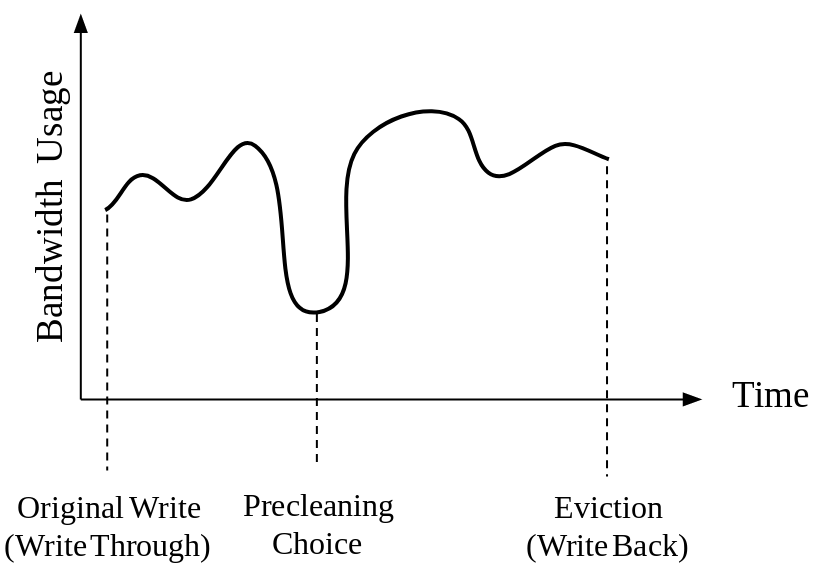
\psfig{file=figs/bandwidth_optimal.eps,height=3.0in}
\caption{Example of cache cleaning choices, showing potential improvement for bandwidth usage.}
\label{f:bandwidth_optimal}
\end{center}
\end{figure}
\index{commands!environments!figure}%

To further improve GPU memory system performance, we would like to use previous data and current memory bandwidth usage levels to know when it’s best to write back modified cache lines. We believe that GPUs are a good fit for this problem due to the parallel nature of the hardware. Making accesses to memory across many cores increases the chances of multiple write-backs being triggered around the same time, this is especially true for data-divergent programs described earlier. GPUs are very reliant on having adequate bandwidth available to hide latency across all cores. When bandwidth saturates, our code will effectively start to serialize, causing us to lose the performance benefits of our parallel architecture. A perfect solution would evenly spread out all write-back traffic, preventing bandwidth spikes that could stall our GPU cores.


\chapter{Background}
\index{Background@\emph{Background}}

\section{GPU Architecture}
\index{GPU Architecture@\emph{GPU Architecture}}
GPUs are highly parallel architectures that aim to always have cores running some useful piece of code. GPUs can be thought of as a CPU with dozens of cores and very quick context switching. As a core stalls for a memory read or write, another warp (analogous to a lightweight process) is scheduled to that core. In this way if the hardware has enough work to schedule across all cores, maximum throughput is achieved and memory latency can be effectively hidden. This GPU model is highly efficient at parallelizing very regular code patterns.

Warps can be broken down even further into threads. Each thread represents a Single Instruction Multiple Data (SIMD) lane [cite?]. The GPU will have dozens of cores running code in parallel, and each individual core will be running 32 or more instances of the same code. SIMD greatly increases the amount of parallelization within the hardware, but, as the name suggests, allows a core to only run a single instruction at a time across its threads. Warps rely on their threads to exhibit regular code and data access patterns. Memory stalls and divergent branch paths within threads both negatively impact performance, effectively serializing parts of the warp. Dynamic warp formation [cite] and memory coalescing [cite?] can help combat code and data divergence respectively, but these techniques cannot completely account for the negative effects of poor code design and inefficient memory access patterns.

Each core on the GPU has a relatively large register file, an L1 cache, and on chip SRAM referred to as shared memory. Each L1 cache is backed by a common L2 cache, which in turn goes to DRAM or global memory. Shared memory can be thought of as per-process memory, it is very fast and solely owned by the warp that allocates it. Global memory is the only way for different warps to communicate. This memory hierarchy helps to alleviate latency of memory accesses. An access to the L1 or L2 cache is much less taxing on warps than waiting on a memory access to DRAM.

\section{Cache Eviction and Replacement}
\index{Cache Eviction and Replacement@\emph{Cache Eviction and Replacement}}
Cache replacement policies are a highly researched and developed area in computer architecture. Least Recently Used (LRU) is often used as a baseline metric in papers because it is easy to reason about and cheaper to implement compared to state of the art replacement policies. However, LRU only learns on very basic information currently within the cache (there are no extra data stores for previously evicted lines). Additionally, LRU is susceptible to very poor performance given pathological access patterns that can cause thrashing. Early attempts to improve LRU such as Qureshi’s et al’s DIP paper \cite{dip} attempt avoid the effects of thrashing by augmenting LRU to randomly insert lines into the Most Recently Used (MRU) position. Over the past couple decades we have seen a trend from heuristic based approaches such as DIP to more theoretically grounded replacement policies like EVA \cite{eva} and Hawkeye.

Belady’s OPT algorithm \cite{belady_opt} is the optimal cache replacement policy assuming no prefetching, identical cost for all misses, and knowledge of the future. When determining what line to evict, OPT chooses the line that will be reused furthest in the future. Belady’s OPT can be used as a ground truth for machine learning algorithms attempting to predict optimal cache replacement choices. In the related work section we will briefly elaborate on how Hawkeye approximates OPT online with the OPTGen algorithm, and we will discuss how OPTGen informs Hawkeye’s replacement decisions.

\section{Deadblock Predictors}
\index{Deadblock Predictors@\emph{Deadblock Predictors}}
Deadblock predictors are a natural evolution of basic replacement policies like LRU [cite]. Deadblock predictors opt to predict what lines will no longer be reused again in the cache rather than using locally greedy decisions like LRU. Deadblock predictors predict on a variety of features such as timestamps of hits, PC of the hit, etc. In particular we will be looking at non-PC based deadblock predictors, as typically LLCs on GPUs don’t have access to PC information (and we’re currently not confident that across so many warps PC would give much information anyways). Deadblock predictors that forego PC information include cache burst and EVA. We find deadblock predictors interesting for the idea of precleaning because we believe they can be used to also help us predict a write that benefits from precleaning.


\chapter{Related Work}
\index{Related Work@\emph{Related Work}}

This report draws upon many different concepts in computer architecture cited above, but the three related works we find the most relevant are Hawkeye’s original publication by Jain and Lin \cite{hawkeye}, Koo et al’s Access Pattern-Aware Cache Management (APCM) paper \cite{apcm}, and two patents by Marvell and Nvidia that are similar to our idea of precleaning \cite{preclean_cpu,preclean_nvidia_patent}.

\section{Hawkeye}
Hawkeye, as touched on in the background section, uses OPTGen as an online method for approximating the optimal cache replacement policy. OPTGen is always trying to match two sequential accesses to a cache line over the program's execution. The time between these sequential accesses represents how long a line needs to be in the cache before getting a hit. With a 4-way associative cache OPTGen can only have 4 of these lines overlapping before a line must be evicted or bypassed. OPTGen, like Belady’s OPT, always prefers lines that has its next access the earliest, and thus prefers caching lines with the shortest interval between accesses. When OPTGen decides to forego caching a line, this line’s associated feature is trained negatively (cache unfriendly), and likewise OPTGen positively trains (cache friendly) features associated with lines that are successfully cached. When Hawkeye needs to evict a cache line it prefers to evict the lines that OPTGen determines to be cache unfriendly. When all lines are cache friendly, Hawkeye falls back on RRIP \cite{rrip} to decide which line to evict.

\section{APCM}
APCM is a relatively recent paper on GPU caching improvements that our research draws draws inspiration from in a number of ways. APCM provides some key insights into the differences between CPU and GPU caches. One of the more interesting points in the paper is its measurement of how sensitive certain GPU benchmarks are to cache performance. Furthermore, APCM also introduces the idea of sampling warps for its replacement policy meta-data. Rather than adding complicated sampling mechanisms to all the L1 caches, APCM instead assumes that GPU programs are regular enough such that a single warp's access patterns is representative of all the other warps. Finally, we note that APCM is notable for this research for affirming the idea that more complicated cache replacement policies can be applied at the L1 without significant performance costs. Typically, we would not see anything more complicated than LRU replacement at the L1 level for latency and cost savings. APCM shows that we can benefit from a relatively more complex scheme at the L1 level.

\section{Precleaning Related Patents}
(Precleaning Patents)


\chapter{Solution}
\index{Solution@\emph{Solution}}


In this section we cover the specifics of both applying Hawkeye to GPU caching and what is required of a cache precleaning system. Our approach for Hawkeye consists of fine tuning the predictor to be more optimized for a GPU environment and evaluating the importance of replacement policies on GPUs. Additionally, we present the basic building blocks required for a cache precleaning system such as a modified deadblock predictor and a bandwidth usage prediction scheme.

\section{Hawkeye on GPU}
Adapting Hawkeye to GPUs requires proper training features, adapting caching mechanisms to support said features, and a basic understanding of the effects of latency on caching performance. We implement Hawkeye with two basic features: the Program Counter (PC) and PC combined with warp ID (PC+WID). Furthermore, we implement and evaluate Hawkeye on both the L1 and L2 cache.

The PC is a very rich feature to train on in CPUs and is a very common feature in CPU cache replacement policies, prefetchers, and branch predictors. However, kernels on GPUs tend to be much smaller and have fewer accesses to global memory compared to processes on CPUs. These factors lead to a much smaller number of PCs that access global memory making it harder to use only PC as a feature for Hawkeye. To alleviate this lack of diversity in PC values, we can include warp ID as an additional feature. If we combine PC with the ID of the warp executing the memory access we can achieve a much more fine grained set of values to train our predictor on. We use Cantor pairing to act as a basic hashing mechanism between our PC and warp ID. While Cantor pairing gives decent performance for how simple it is, we believe Cantor pairing may be inefficient in hardware because of the multiplication step involved.

Typically, on CPUs, complex cache replacement policies are reserved for last level caches where high latency is expected and more memory is available for storing meta-data. However, as we’ve seen in implementations like APCM, L1 caches on GPUs can actually have complex replacement policies while still seeing performance benefits. GPU on-chip memory is shared between the register file, shared memory, and L1 cache and can be used to store meta-data for our replacement policies. The additional meta-data required to implement Hawkeye can come both from the L1 cache itself or additional memory can be repurposed from the register file and shared memory if needed. Furthermore, because GPUs are inherently dependent on throughput and not latency, slight increases in latency at the L1 level don’t negatively impact performance as much on GPUs as they would on CPUs.

\section{Cache Precleaning}

To successfully hide write traffic, a proper solution requires two important predictions: predicting the final write to a line, and predicting the optimal time to commit our precleans. Given a trace of the program from previous executions, one could perfectly reorder writes to minimize the impact writes have on our memory systems. Our goal when designing some cache precleaning unit is to predict what lines are dirty but will not be written to again until eviction. When we know what lines we can preclean, we need to predict if the current cycle is the best time to clean our line, or if there may be an even lower bandwidth usage point in the future.  

\subsection{Final Line Write Prediction}
Deadblock predictors are useful for precleaning because they give us an idea of active a line currently is. It's very likely that we would want to preclean a line that is a deadblock, because said line is predicted to have no reads or writes in the future. Though we would like to be more accurate than this, we would like to predict when a line is a deadblock for the purposes of writes but is still being accessed by reads. We are in some ways trying to predict the future state of the cache. We would like to predict what is most likely to be the next evicted line with missing information such as all the series of accesses leading up to the eviction. We believe we can modify a deadblock predictor to predict our precleaning candidates by finding when the final write for a line is executed.

\subsection{Bandwidth Variation and Prediction}
A common code pattern in GPU programs is to load data in from global memory into shared memory, do parallel computations, then write back the result of the computations to global memory. Because of the nature of parallel programming, there are often times when different computation units need to synchronize and wait for all other units before continuing. A convenient time to do this synchronization is right after our cores write back to global memory. This synchronization ensures that all threads see the latest state of computation before continuing. Please refer to Figure \ref{f:cuda_sync} for basic pseudo-code that shows this coding pattern.

\begin{figure}[htb]
\begin{center}

\begin{lstlisting}
for (int i = 0; i < N; i++) {
  int new_data_idx = getNextPieceOfData(threadIdx);
  int* data = global_data[new_data_idx];
  doComputations(data);
  global_data[new_data_idx] = *data;
  syncThreads();
}
\end{lstlisting}
\caption{Pseudo-code for common synchronization code pattern in CUDA code.} This data is loaded in from DRAM (as this is the only way data can be shared across cores on a GPU) to local shared memory. When computations are done and stored back to global memory, we need to manually synchronize to prevent race conditions in the data.
\label{f:cuda_sync}
\end{center}
\end{figure}
\index{commands!environments!figure}%

%Figure 2: Here we load in data assigned to our current thread (which may or may not change as the program goes on). This data is loaded in from DRAM (as this is the only way data can be shared across cores on a GPU) to local shared memory. When computations are done and stored back to global memory, we need to manually synchronize to prevent race conditions in the data.

This synchronization technique yields a very useful bandwidth pattern for our technique of precleaning. As cores hit the synchronization barrier their bandwidth usage will drop off, making the synchronization point an opportune time to send out write backs. Furthermore, because these synchronization points are clearly defined in the code, it becomes very easy to predict when they are coming. We also see much more pronounced dips in bandwidth usage between executions of kernels, though kernel termination happens much less often compared to thread synchronization.


\chapter{Experiments and Headroom}
\index{Experiments and Headroom@\emph{Experiments and Headroom}}

For our experiments we used GPGPUsim with a variety of programs from the Rodinia 2.0 and Lonestar 2.0 benchmark suites. Later in this section, we present promising results for applying Hawkeye to our GPU simulator environment. However, due to the lack of both time and domain knowledge, we were only able to gather basic headroom data for our idea of cache precleaning. In the following sections we will describe the details of the simulator used, discuss properties of our benchmarks and platform such as cache sensitivity and bandwidth usage, and finally present our headroom and actual performance improvements using Hawkeye and precleaning.

\section{Simulator}
We use the GPGPUsim \cite{gpgpusim} simulator for our experiments, targeting the provided configuration that approximates the Nvidia Fermi architecture. This architecture supports 15 cores, each core consisting of 32 SIMD lanes and a maximum of 48 scheduled warps. Each core has a private 16 KB, 4-way set associative L1 cache with 128 bytes lines, and the entire system has a shared 786 KB, 8-way set associative L2 cache with 128 byte lines. The L2 cache is split into 12 portions and assigned to the 12 separate DRAM memory partitions. Finally, the L1 cache acts as write-through cache while the L2 cache acts as a write-back cache. A full list of relevant specifications can be seen in Table X [still to-do].

GPGPUsim runs CPU code natively, then intercepts CUDA library calls in order to perform full functional simulation (as opposed to a trace-based simulation). Because GPGPUsim doesn’t provide an option for trace-based simulation, we cannot skip warmup cycles and our simulations take significant amount of time to run to completion. Due to these restrictions, our simulations were sometimes cut short and compared against a baseline that ran for the same amount of time. Unfortunately this means that our results are often extrapolated and could be inaccurate.

The version of GPGPUsim used is a slight modification of the 3.0 release that has basic support for CUDA 5.5. This modified version is used in order to be able to run the Lonestar 2.0 benchmark suite. Furthermore, we made use of the AerialVision \cite{aerialvision} visualization software provided with GPGPUsim, but we made minor modifications in order to display the precleaning data presented in this report.

The baseline caches used within the simulator are all managed by a standard implementation of LRU (no pseudo timestamps are used). Furthermore, as is common on GPUs, the caches have no prefetching and they only cache global reads/writes (accesses to shared memory are on chip and are thus equivalent to an L1 access). All atomic operations skip the L1 cache, and writes cause evictions from the L1 cache.

\section{Cache Sensitivity}
Cache sensitivity tells us how much cache performance affects a given benchmark. We would expect that a benchmark with heavy code divergence or a small memory footprint would have little to no improvements even from an optimal cache implementation. By enlarging the cache and measuring the change in instructions per clock (IPC) over our baseline, we can get a rough approximation of how much a given benchmark relies on the cache. If we see little to no improvement when enlarging the cache, we wouldn't expect a change in replacement policy to have much affect on performance either. Benchmarks with large IPC improvements have high cache sensitivity and benchmarks that do roughly the same as baseline are considered to have low cache sensitivity. In our Hawkeye experiments, we would like to see large performance improvements on benchmarks that have high cache sensitivity, but see performance on par with LRU in benchmarks with low cache sensitivity. This experiment was motivated by the same study done by the APCM paper as referenced in our Related Work section earlier.

In order to measure L1 cache sensitivity we quadrupled the size of our L1 cache and compared IPC performance against our baseline cache described above. We also repeated this experiment for our L2 cache. Our results for this experiment are presented below in Figure \ref{f:sensitvity}. Interestingly enough, we see that a number of graph algorithms including MST, SSSP, and BFS exhibit high levels of cache sensitivity. Graph algorithms on GPU tend to do poorly due to their irregular and hard to predict access patterns. The other interesting thing to note here is that between two runs of bfs we see different levels of cache sensitivity, this could be due to how the two data sets were generated or the differing sizes of the data sets. Another interesting thing to note is when increase the cache size for some of our benchmarks we actually perform even worse. We believe this strange result can be explained by Belady’s anomaly \cite{belady_anomaly}.

\begin{figure}[htb]
\begin{center}
\ 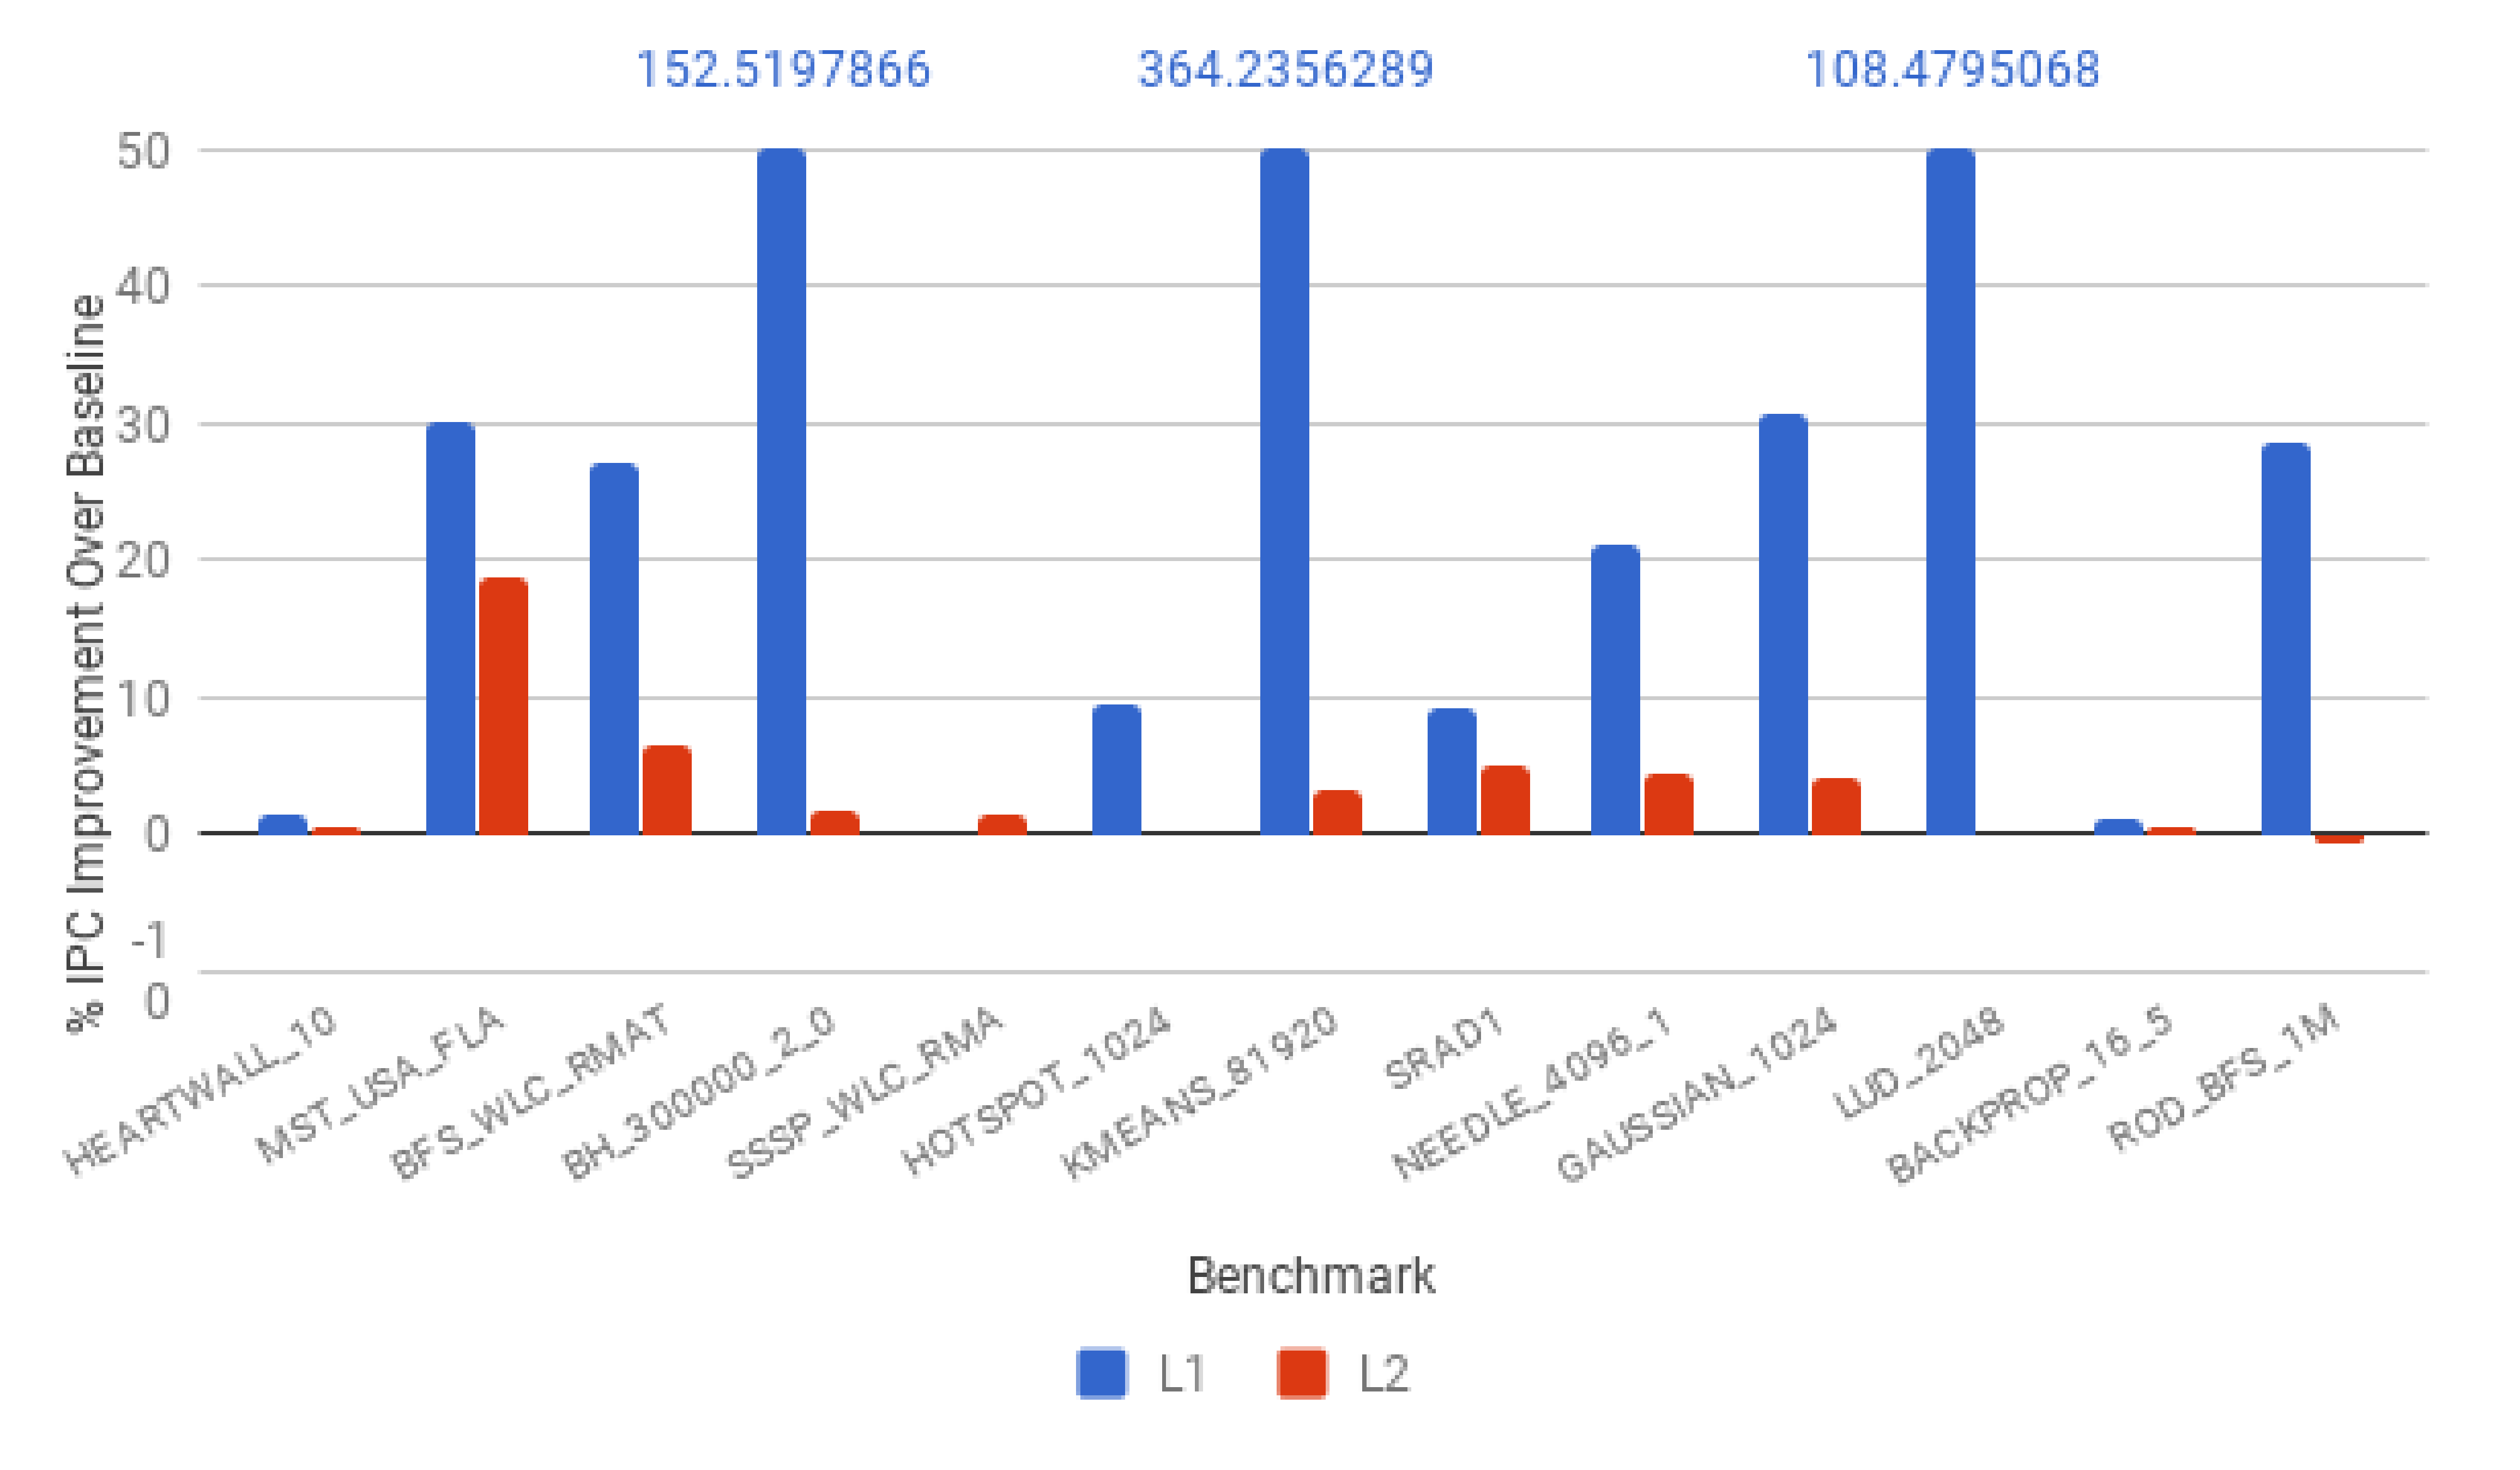
\psfig{file=figs/sensitivity.eps,height=3.0in}
\caption{Cache sensitivity for both L1 and L2 caches.} These numbers are percentage improvements over in IPC over baseline when quadrupling the size of each cache. Replacement for all cases is done with LRU.
\label{f:sensitivity}
\end{center}
\end{figure}
\index{commands!environments!figure}%

\section{Hawkeye}
For evaluating Hawkeye on GPU we first evaluate both PC and PC combined with warp ID as training features by comparing prediction biases. Next we evaluate real performance impact by measuring the change in IPC over our LRU baseline. Overall, we find that Hawkeye does well compared to LRU, though there is no clear winner between our PC and PC+WID features.

To begin, we measured the per-feature bias of the OPTGen algorithm for both the PC and PC+WID features. Per-feature bias essentially tells us the prediction quality of our chosen feature, it tells us how often our predictions on a feature agree with each other. We note that the two hotspot benchmarks have a 100\% per-feature bias. We believe this high bias is caused by a well optimized code base that provides a small amount of PC values (a max of 4 in our simulations). The full set of per-feature biases can be seen in Figure \ref{f:feature_bias}.

\begin{figure}[htb]
\begin{center}
\ 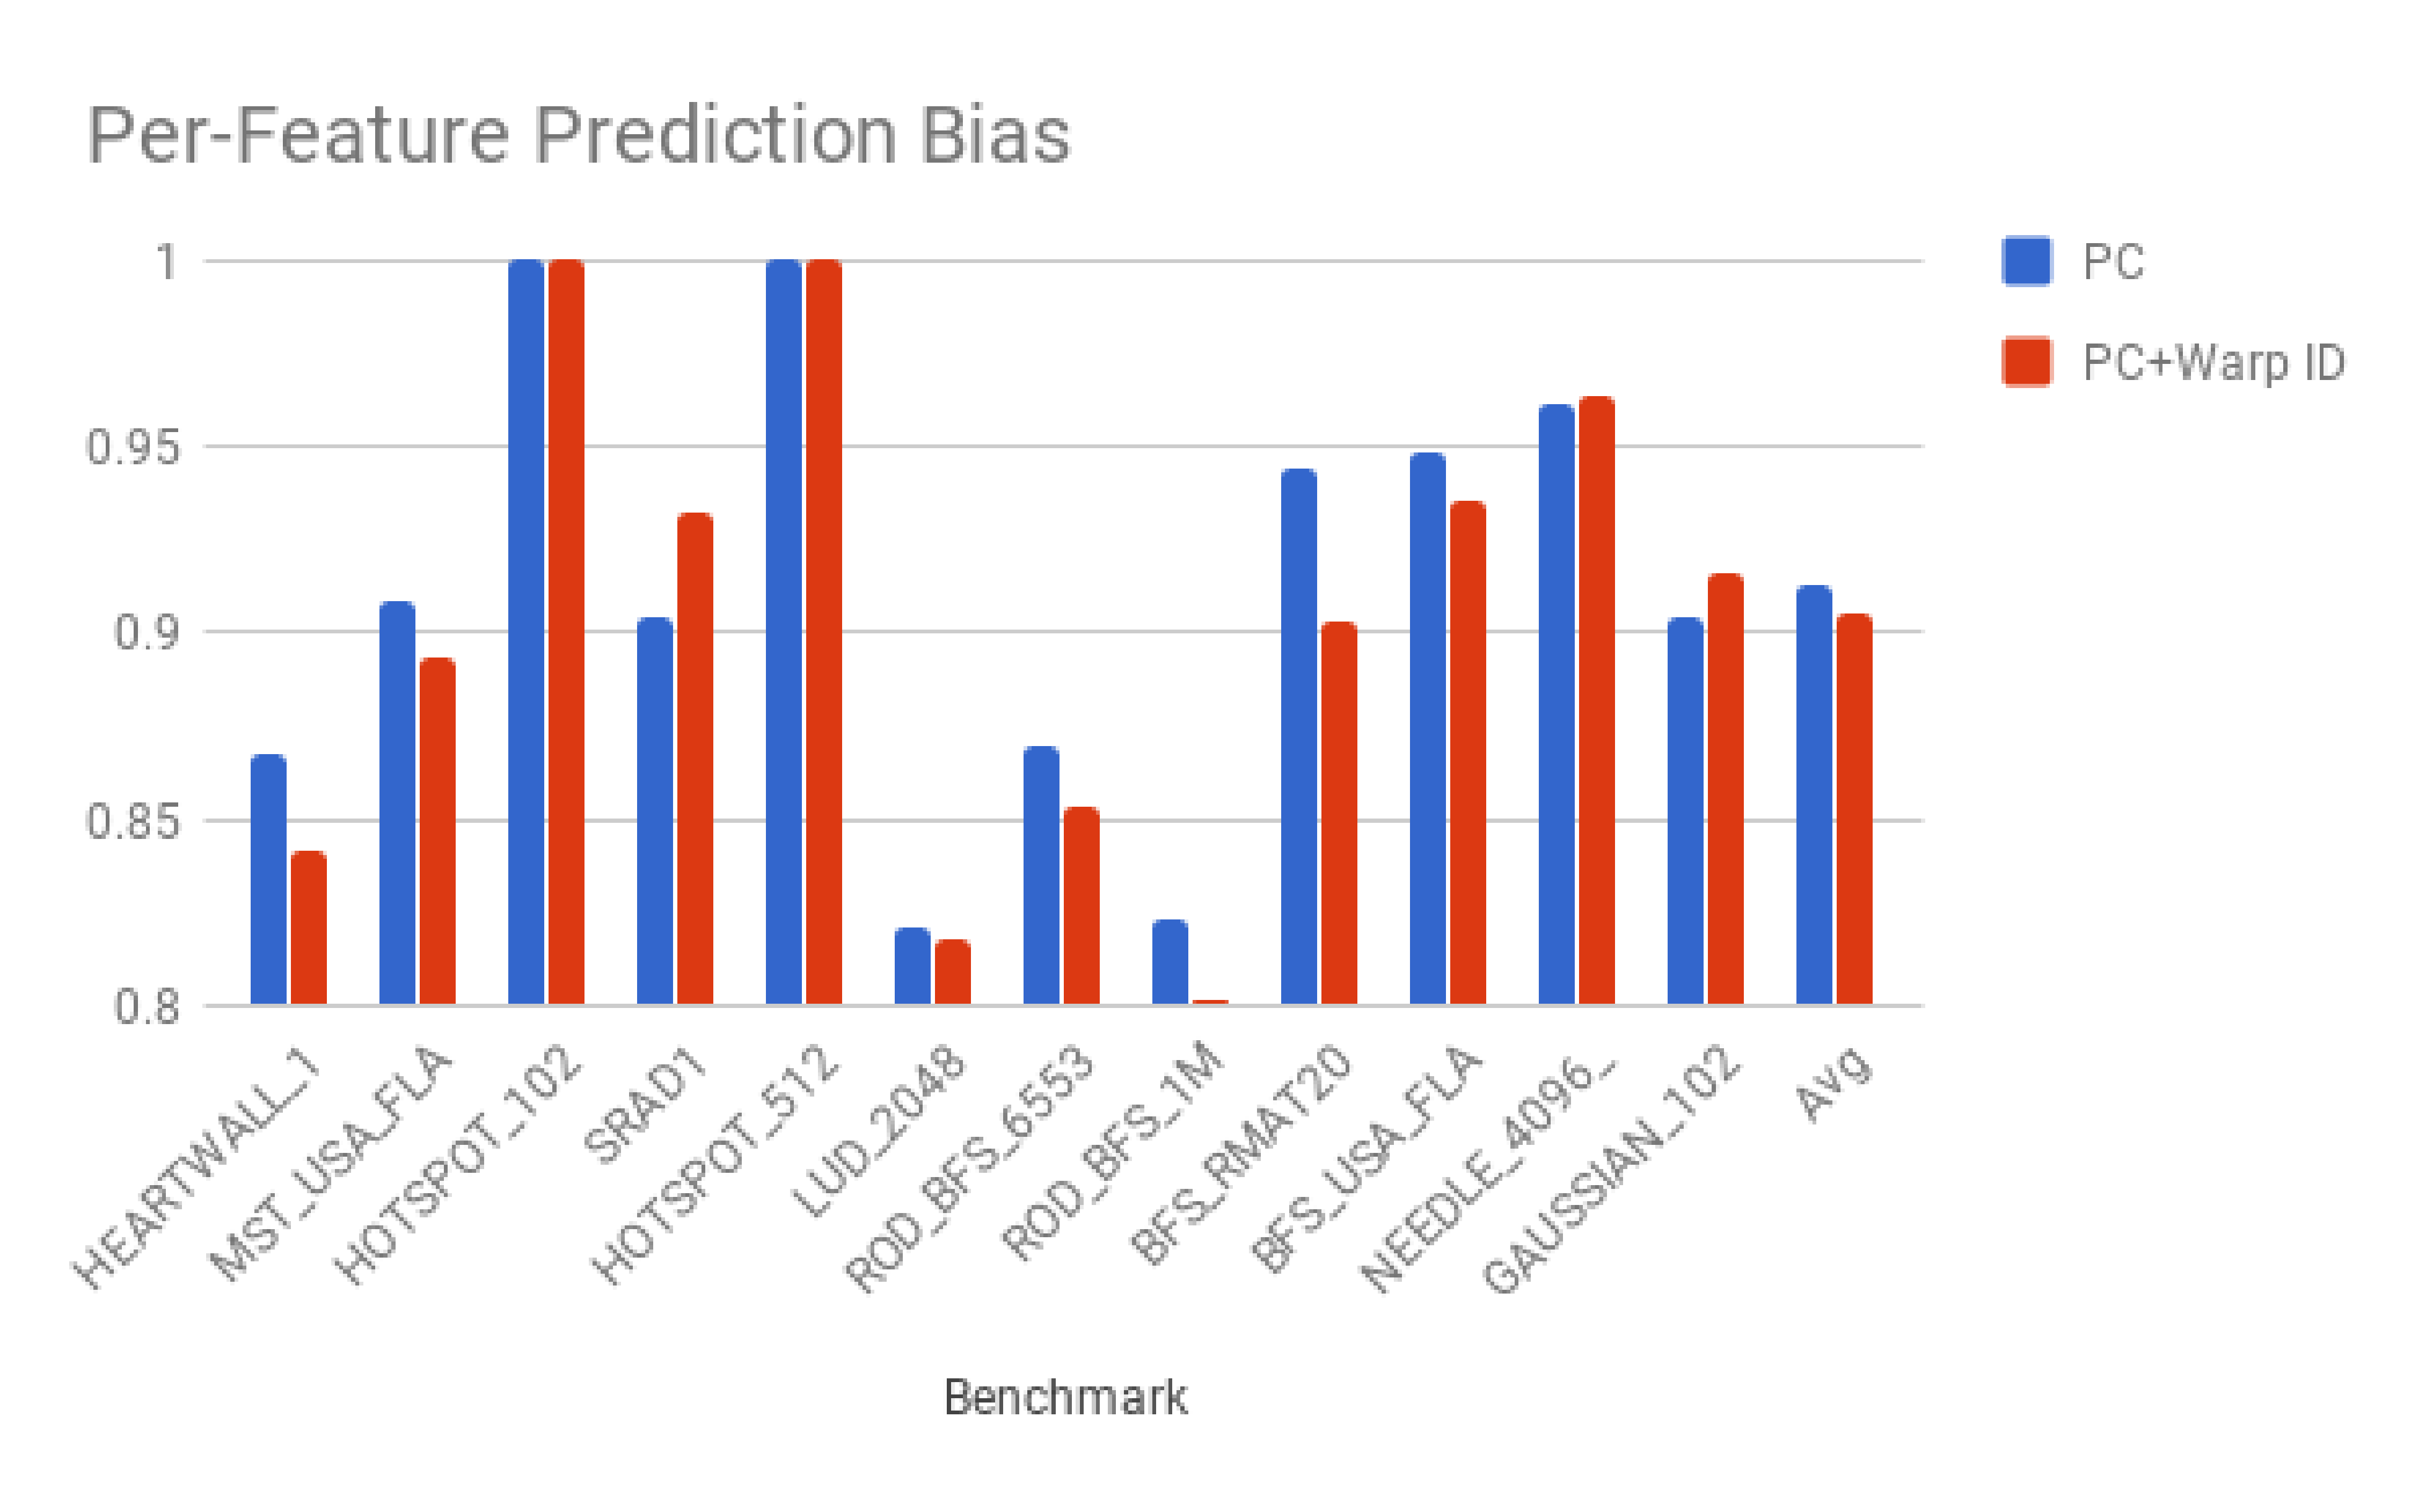
\psfig{file=figs/per_feature_bias.eps,height=3.0in}
\caption{Average per-feature prediction bias.}
\label{f:feature_bias}
\end{center}
\end{figure}
%Figure 5: Average per-feature bias for a variety of benchmarks, evaluated for PC and PC hashed with Warp ID features. Here the y-axis determines how useful our feature is for predicting on. The bias denotes the percentage of truth values that agree with our predicted value of cache friendly or unfriendly. Here 50\% would be equivalent to a random prediction. The final column denotes our average per-feature bias across all benchmarks.

While we see that using PC alone does slightly better on average compared to PC+WID, we will show that this does not necessarily correlate with real world prediction performance. In Figure \ref{f:opt_uniq_vals} is a plot of the number of unique values seen per feature. We believe that PC+WID is preferable in some cases because the more diverse feature values allow us to capture more complicated patterns. Though it is important to note that this large increase in feature values requires adequate hardware to track, and more values being trained typically leads to slower training times. From these results, we believe there is more room for feature experimentation, especially involving dynamic warp IDs or better hashing algorithms.


\begin{figure}[htb]
\begin{center}
\ 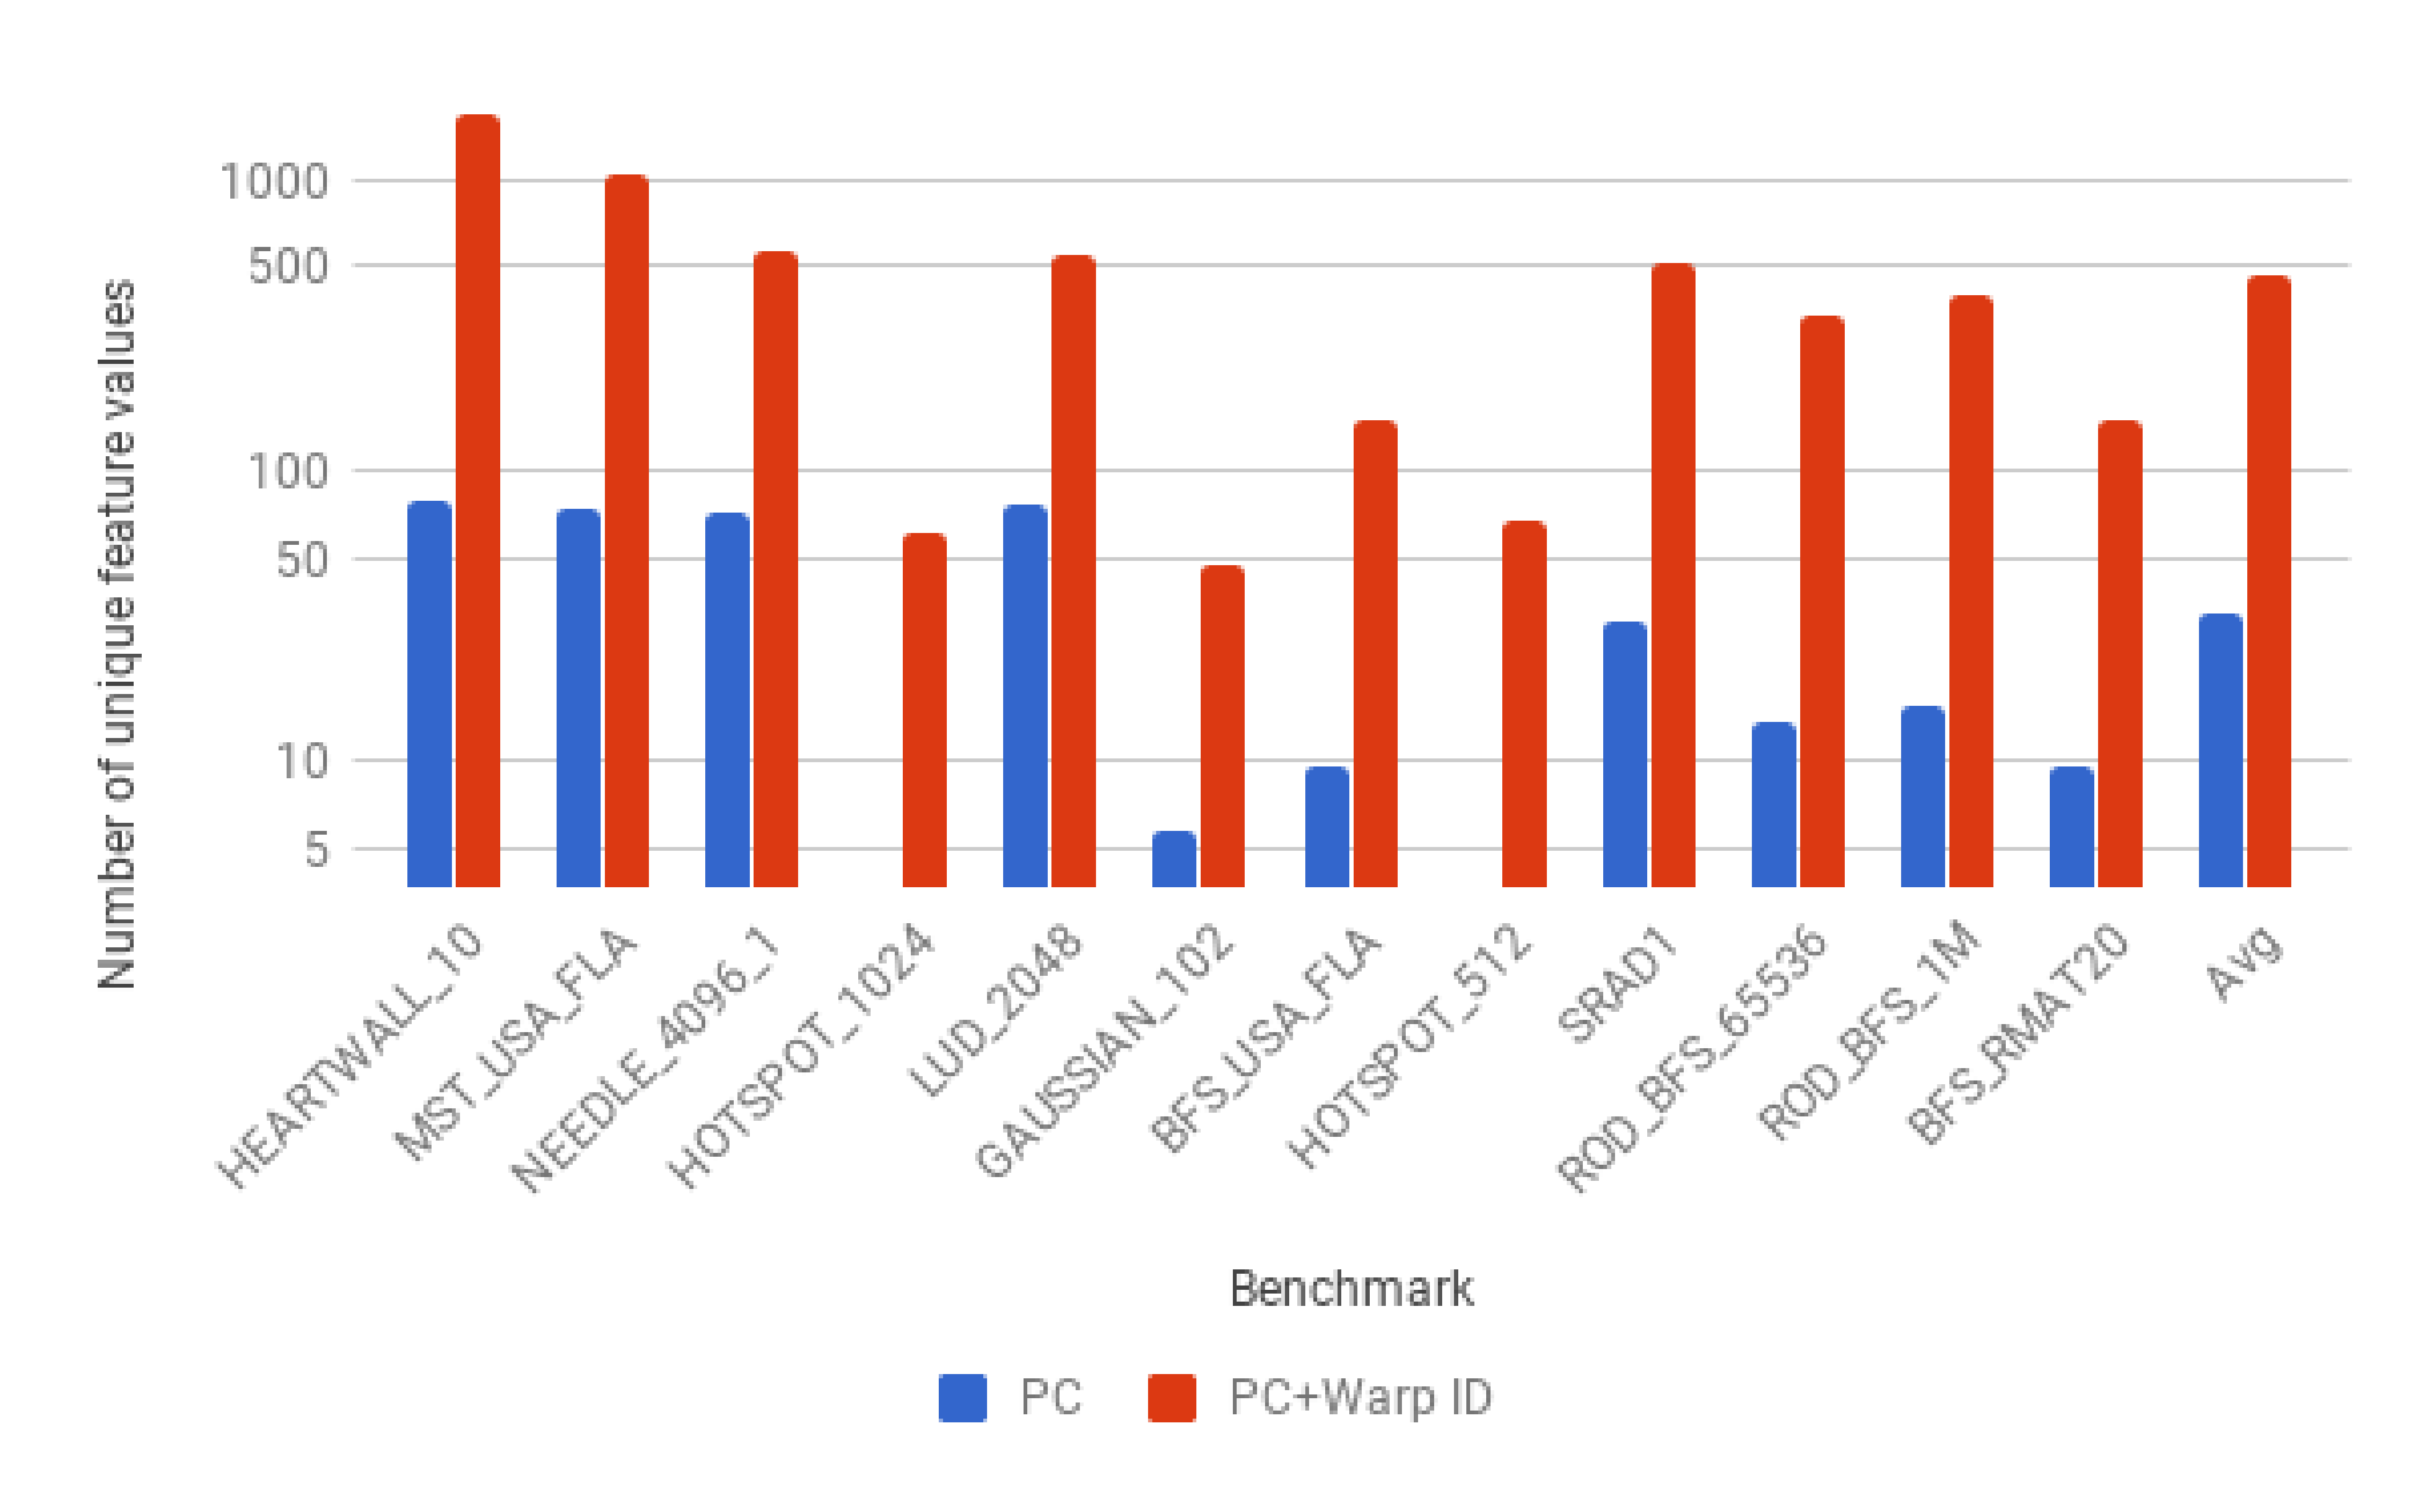
\psfig{file=figs/opt_uniq_vals.eps,height=3.0in}
\caption{Average unique values per feature.}
\label{f:opt_uniq_vals}
\end{center}
\end{figure}
%Figure 6: Average unique values per feature. This is a rough measure of the variance of our features on each benchmark. We would ideally see a feature with high spread and high bias.

In our full performance tests we measured two important metrics: post-warmup cache miss rate, and IPC improvement over baseline. For the post-warmup miss rate metric, we ignore all cache misses before a specified warmup time, as most misses at the beginning of a program are compulsory and cannot be avoided. We found that a post-warmup time of 3,000,000 cycles fits most of the benchmarks being used (with the exception of HOTSPOT which ends before 3,000,000 cycles). We present the miss rate improvement over LRU in Figure \ref{f:hawkeye_pw_miss_rate}. As mentioned above, PC hashed with warp ID ends up performing better than just PC.


\begin{figure}[htb]
\begin{center}
\ 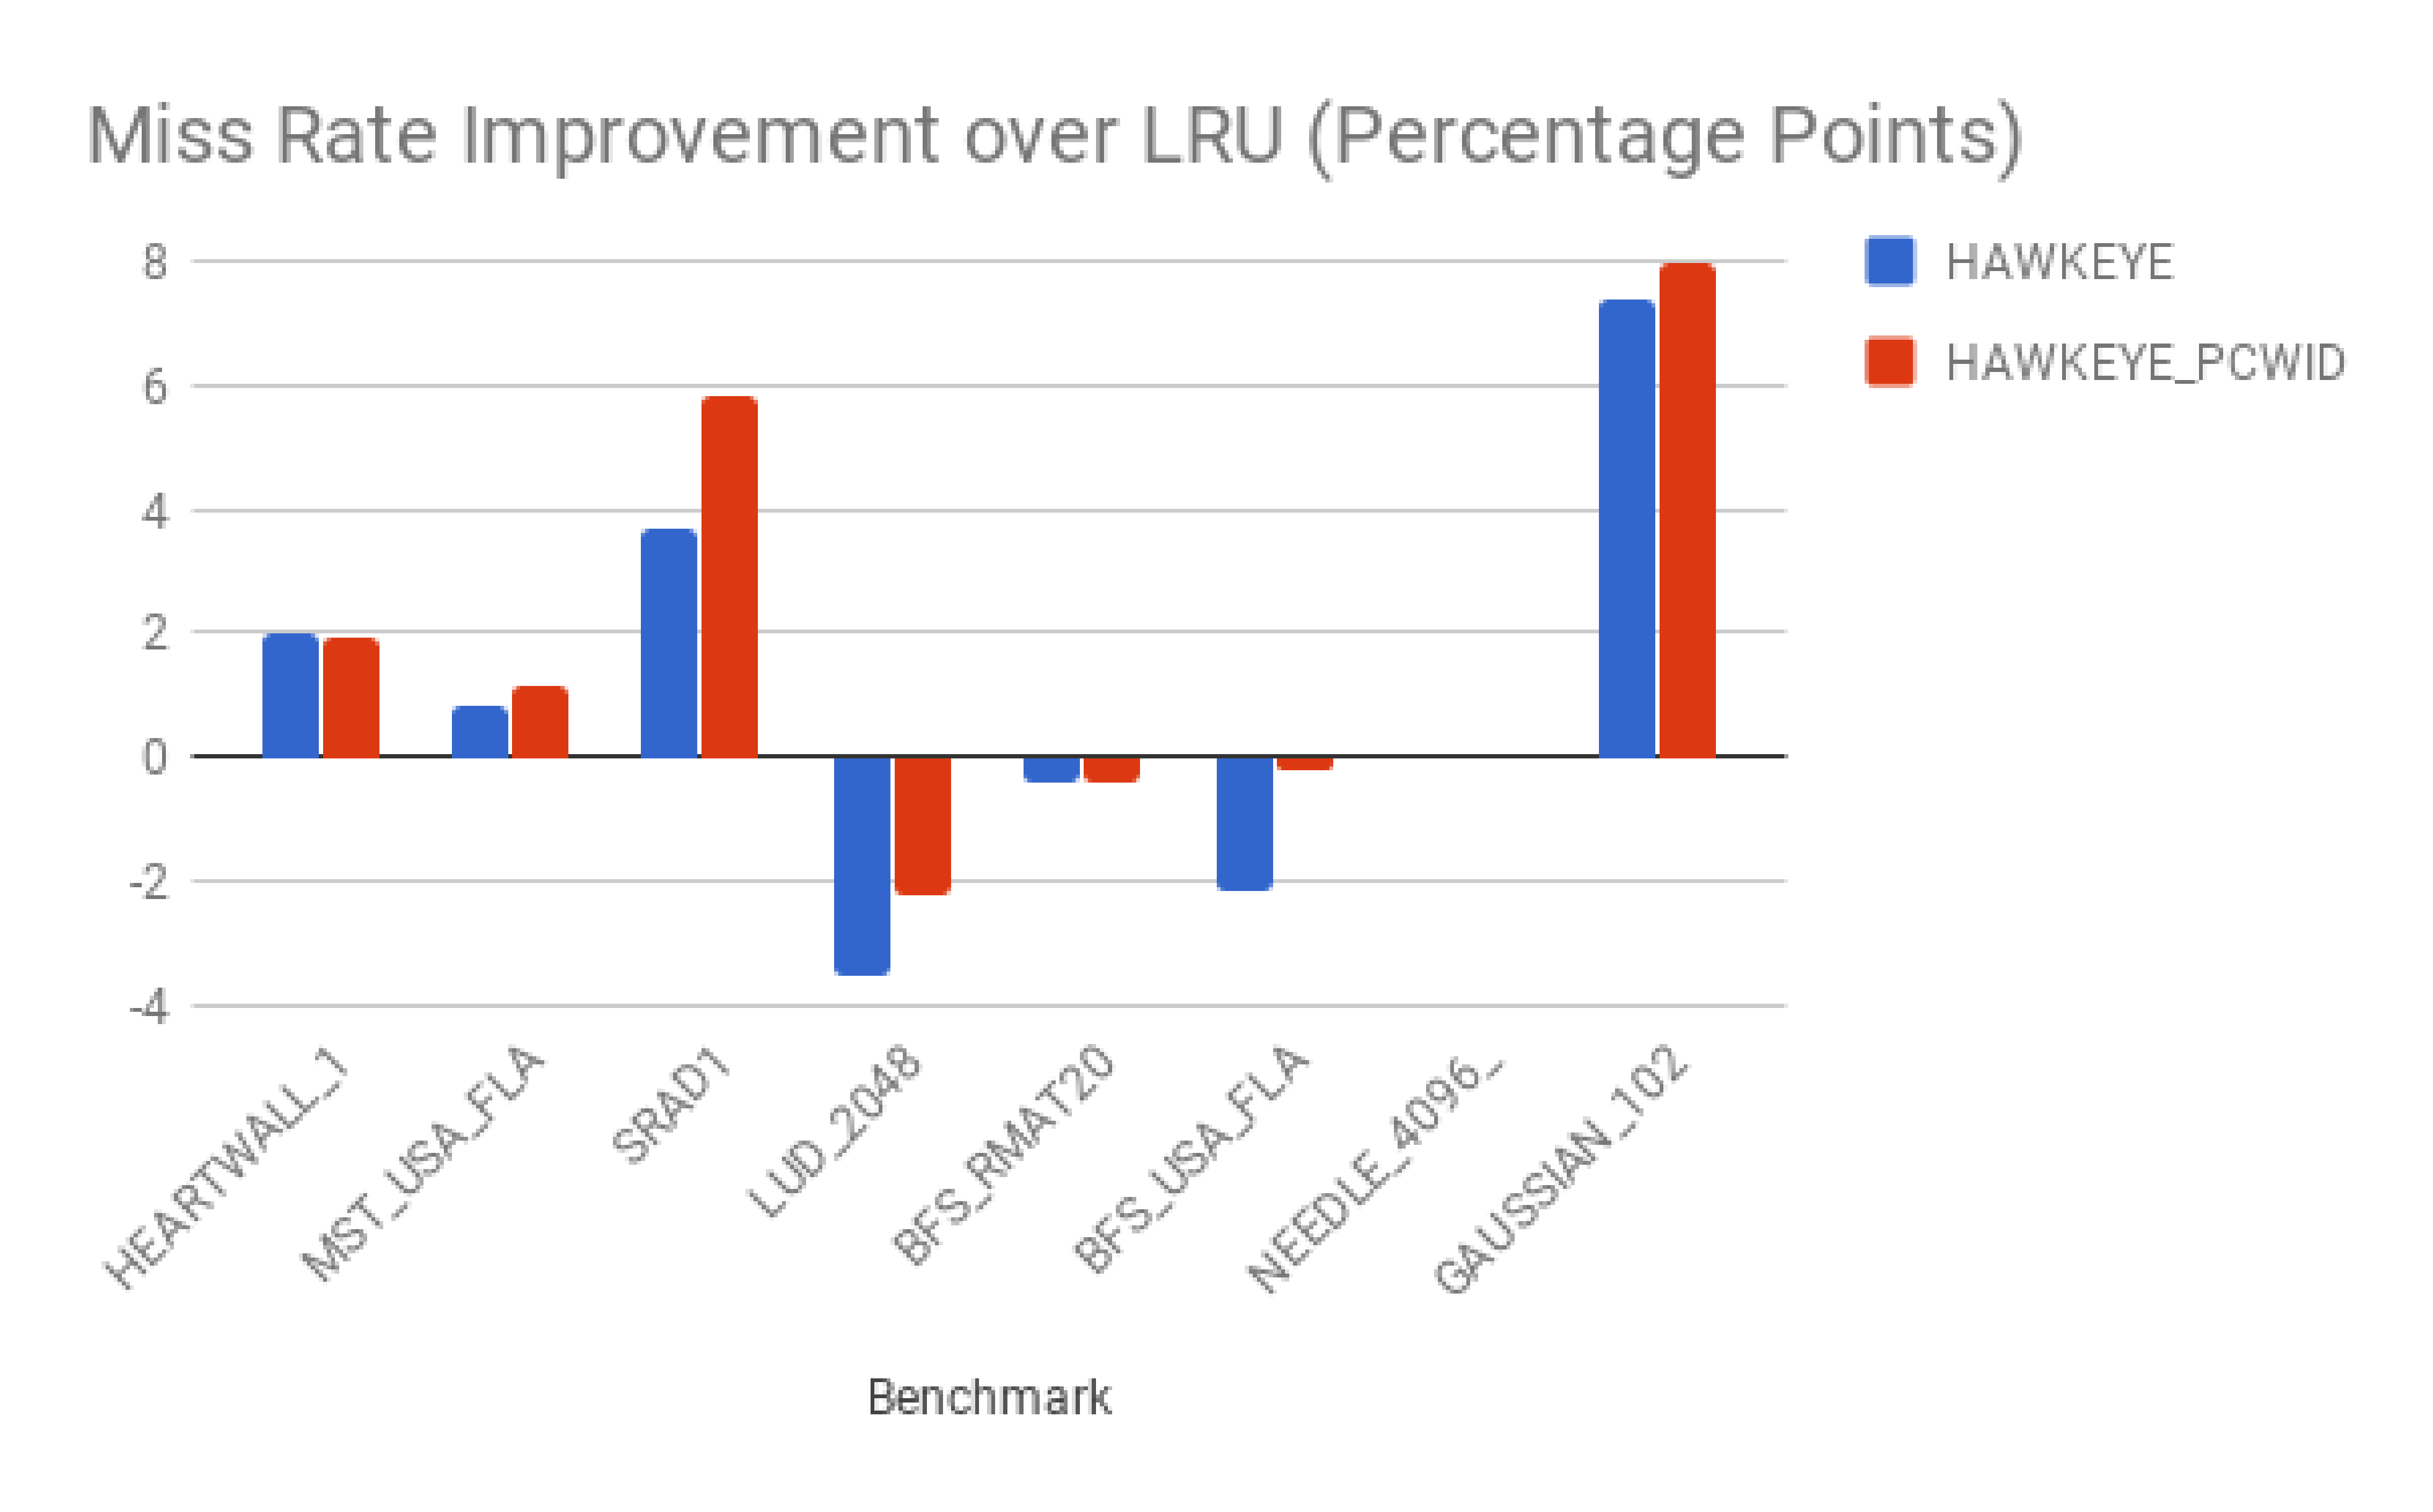
\psfig{file=figs/hawkeye_pw_miss_rate.eps,height=3.0in}
\caption{Miss rate improvement over LRU (percentage points).}
\label{f:hawkeye_pw_miss_rate}
\end{center}
\end{figure}
%Figure 7: Miss rate improvement over LRU. This improvement is measured in percentage points over the miss rate observed with LRU.

\section{Precleaning}


\chapter{Future Work and Remarks}
\index{Future Work and Remarks@\emph{Future Work and Remarks}}



\chapter{Conclusion}

In this research report we evaluated the cache replacement policy Hawkeye on GPUs and provided coarse headroom for the idea of precleaning. We believe both of these ideas can provide benefits to GPU performance, but current implementations are fairly situational and require the code being run to be sensitive to caching performance and bandwidth usage. We conclude that Hawkeye will provide the most benefit when applied at the L1 cache with just PC as the feature for OPTgen. However, from our sensitivity study, we believe there's more room for improvement at both the L1 and L2 caching replacement policies. Furthermore, our idea of precleaning requires more sophisticated predictors and metrics before it can be fully evaluated.


%\include{chapter-introduction}
%
%\include{chapter-instructions}
%
%\include{chapter-howtouse}
%
%\include{chapter-makingbib}
%
%\include{chapter-tables+figs}
%
%\include{chapter-math}


%%%%%%%%%%%%%%%%%%%%%%%%%%%%%%%%%%%%%%%%%%%%%%%%%%%%%%%%%%%%%%%%%%%%%%
% Appendix/Appendices                                                %
%%%%%%%%%%%%%%%%%%%%%%%%%%%%%%%%%%%%%%%%%%%%%%%%%%%%%%%%%%%%%%%%%%%%%%
%
% If you have only one appendix, use the command \appendix instead
% of \appendices.
%
%\appendices
%\index{Appendices@\emph{Appendices}}%
%
%\include{chapter-appendix1}
%
%\include{chapter-appendix2}
%
%\include{chapter-appendix3}

%%%%%%%%%%%%%%%%%%%%%%%%%%%%%%%%%%%%%%%%%%%%%%%%%%%%%%%%%%%%%%%%%%%%%%
% Generate the index.						     %
%%%%%%%%%%%%%%%%%%%%%%%%%%%%%%%%%%%%%%%%%%%%%%%%%%%%%%%%%%%%%%%%%%%%%%
%								     %
% NOTE: For master's theses and reports, NOTHING is permitted to     %
%	come between the bibliography and the vita. This section     %
%	to generate the index (if used) MUST be moved to before      %
%	the bibliography section.				     %
%								     %
%\printindex%    % Include the index here. Comment out this line      %
%		% with a percent sign if you do not want an index.   %
%%%%%%%%%%%%%%%%%%%%%%%%%%%%%%%%%%%%%%%%%%%%%%%%%%%%%%%%%%%%%%%%%%%%%%

%%%%%%%%%%%%%%%%%%%%%%%%%%%%%%%%%%%%%%%%%%%%%%%%%%%%%%%%%%%%%%%%%%%%%%
% Generate the bibliography.					     %
%%%%%%%%%%%%%%%%%%%%%%%%%%%%%%%%%%%%%%%%%%%%%%%%%%%%%%%%%%%%%%%%%%%%%%
%								     %
% NOTE: For master's theses and reports, NOTHING is permitted to     %
%	come between the bibliography and the vita. The command      %
%	to generate the index (if used) MUST be moved to before      %
%	this section.						     %
%								     %
\nocite{*}      % This command causes all items in the 		     %
                % bibliographic database to be added to 	     %
                % the bibliography, even if they are not 	     %
                % explicitly cited in the text. 		     %
		%						     %
\bibliographystyle{plain}  % Here the bibliography 		     %
\bibliography{preclean}        % is inserted.			     %
\index{Bibliography@\emph{Bibliography}}%			     %
%%%%%%%%%%%%%%%%%%%%%%%%%%%%%%%%%%%%%%%%%%%%%%%%%%%%%%%%%%%%%%%%%%%%%%


%%%%%%%%%%%%%%%%%%%%%%%%%%%%%%%%%%%%%%%%%%%%%%%%%%%%%%%%%%%%%%%%%%%%%%
% Vita page.							     %
%%%%%%%%%%%%%%%%%%%%%%%%%%%%%%%%%%%%%%%%%%%%%%%%%%%%%%%%%%%%%%%%%%%%%%

%\begin{vita}
%Craig William McCluskey
%was born in Minneapolis, Minnesota on 20 May 1950, the son of
%Dr. William R. McCluskey and Lucilla W. McCluskey.  He received the Bachelor
%of Science degree in Engineering from the California Institute of Technology
%and was commissioned an Officer in the United States Air Force in 1971.
%He entered active duty in October, 1971, and was stationed in Denver, Colorado,
%Colorado Springs, Colorado, Panama City, Florida, and Sacramento, California.
%He separated from the USAF in 1975 and worked as an engineer for several small
%electronics companies in California before moving to Colorado Springs, Colorado
%to work for Hewlett-Packard in 1979. He left Hewlett-Packard in 1989 and joined
%a small company based in Herndon, Virginia, working out of his house as a
%``remote'' engineer designing parts of the Alexis satellite for Los Alamos
%National Laboratories. Laid off when his portion of the satellite was
%completed, he applied to the University of Texas at Austin for enrollment
%in their physics program. He was accepted and started graduate studies in
%August, 1991.
%
%\end{vita}

\end{document}
